\documentclass[DM,lsstdraft,toc]{lsstdoc}

% Package imports go here

% Local commands go here

\title[Deblender Data Products]{Proposal for Deblender Outputs as Level 2 Data Products}

\author{
James~Bosch
}

\setDocRef{LDM-513}
\date{\today}
\setDocRevision{1}
\setDocStatus{draft}

\setDocAbstract{%
Most catalog measurements produced in a LSST Data Release Production will be derived from pixel values that have been \emph{deblended} -- we have apportioned the flux in each pixel to each of the \Objects that overlap that pixel.  These deblended pixels values are thus a critical link in our provenance chain, and should be provided to users as a first-class data product.  This document provides further justification for the proposal to add this data product and provides a preliminary estimate of the impact on data storage requirements of an additional $83\,\mathrm{TB}$ in DR1 and $221\,\mathrm{TB}$ in DR11.
}

% Change history defined here. Will be inserted into
% correct place with \maketitle
% OLDEST FIRST: VERSION, DATE, DESCRIPTION, OWNER NAME
\setDocChangeRecord{%
\addtohist{1}{2017-04-01}{Initial release.}{James Bosch}
}

\begin{document}

% Create the title page
% Table of contents will be added automatically if "toc" class option
% is used.
\maketitle

\section{Introduction}

Essentially all measurements in LSST's \Object table (\DPDD) are directly or indirectly derived from running the ``deblender'' algorithm on coadd images.  The deblender apportions the flux in each pixel between the \Objects that overlap that pixel (with \Object extent defined by a surface-brightness threshold).  Subsequent measurements on the coadds themselves use a combination of the original pixels and the deblended pixels as their inputs.  We will also use the deblended pixels indirectly for Forced \Source measurements and the Bulge-Disk Model and Moving Point \Source Models that are fit to individual per-epoch images, as these measurements will be initialized from coadd processing and may utilize per-epoch deblended pixels that are computed from the deblended coadd pixels.

These deblended pixel values are thus a critical link in the provenance change between the coadd images and the measurements in the \Object and \ForcedSource tables.  DM developers and science users (especially those interested in rare \Objects) will need to access deblended pixel values to understand any measurement outliers that may be due to deblending problems.

Deblended pixel values are also an important input to Level 3 algorithms that perform new measurements on individual \Objects.

The deblender itself is a compuationally expensive algorithm that will run simultaneously on multiple coadds.  It will likely use some combination of \emph{deep} and \emph{best-seeing} coadds, but it may utilize \emph{short-period} or \emph{PSF-matched} coadds as well.

We also run a variant of the deblender on visit-level images prior to running the measurements that populate the \Source table.  This variant requires only the CCD-level Processed Visit Image as input.

\section{Proposal and Implementation Options}

We propose adding deblended \emph{deep} coadd pixel values (in each band) for each \Object as a first-class Level 2 data product.  Our recommendation for the data structure for this information is one \texttt{HeavyFootprint} for each \Object.  A \texttt{HeavyFootprint} combines a run-length encoding of the region covered by an \Object (which we call a \texttt{Footprint}) with a 1-d array of 32-bit floating point values containing just the pixels in that region.  \texttt{Footprint}s themselves are small: three 32-bit integers for each pixel \emph{row} in the region.  \Objects that were not deblended (because they had no neighbors) need only have a \texttt{Footprint}; their \texttt{HeavyFootprint} can be generated on-the-fly efficiently from the \texttt{Footprint} and the coadd images.

Despite the fact that they are tied to \Objects, the access patterns for \texttt{HeavyFootprints} should be assumed to be more coupled to the access patterns for coadd images, but will be even less frequent: users who request \texttt{HeavyFootprints} will almost always want coadd images as well (though the converse is not true).  We anticipate that in most cases, these requests will be for single \Objects (and cut-outs of coadd images near them), not all \Objects in a field.

We do not believe regenerating \texttt{HeavyFootprint}s by re-running the deblender on-demand is a viable way to implement this proposal; even if running it does not require regenerating some coadds, the deblender will still likely be one of our most computationally expensive algorithms, and we currently have no requirement to make it executable on a per-\Object bases.  So while regenerating \texttt{HeavyFootprints} may technically represent a tradeoff between computation and storage, it likely the storage cost will be sufficiently lower (as well as lower-latency).  The deblender algorithm \emph{may} permit a highly compressed output (e.g. an analytic model) that allows the true \texttt{HeavyFootprints} to be regenerated from the coadd data (which would be an acceptable implementation), but this cannot be guaranteed today.

We do not propose storing \texttt{HeavyFootprints} for \emph{best-seeing} or other coadd flavors besides \emph{deep}.  It is likely these could be derived efficiently from those coadd images and the \emph{deep} coadd \texttt{HeavyFootprints}, but since most measurements will be done on the \emph{deep} coadds we anticipate the need for deblender outputs for other flavors to be much less.

We also do not propose storing \texttt{HeavyFootprints} for \Source.  We expect {\Source measurements to be much more lightly used than \Object or \ForcedSource measurements, and \Source \texttt{HeavyFootprints} can be more efficiently regenerated because they are produced by a simpler, faster form of the deblender.

\section{Impact on Storage}

Because the pixels included in the set of \texttt{HeavyFootprints} are defined by a surface-brightness threshold, the storage costs for \texttt{HeavyFootprints} are a function of depth.  We have attempted to estimate this scaling by using LSST DM Stack processing of Hyper-Suprime Cam Subaru Strategic Program Survey (HSC SSP) data \citep{2017arXiv170208449A}.  The HSC SSP data includes both a Wide layer ($1200\,s$ in $i$) and an UltraDeep layer ($9000\,s$ in $i$ to date).

\begin{figure}
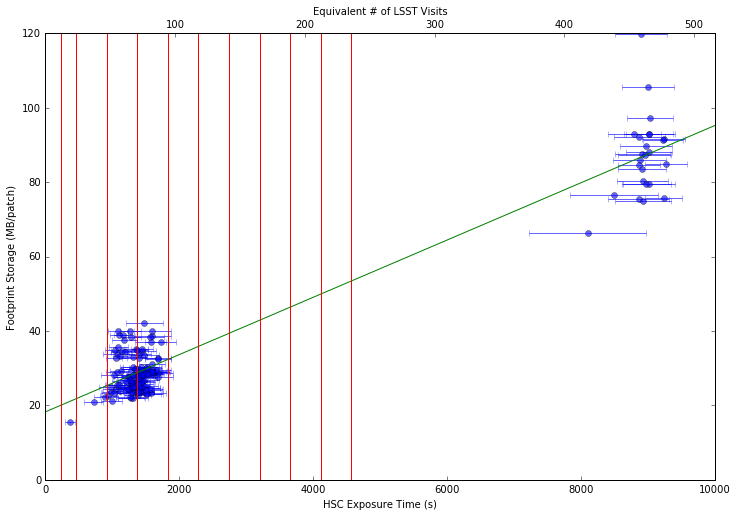
\includegraphics[width=\textwidth]{regression.png}
\caption{Per-patch \texttt{HeavyFootprint} storage costs in LSST processing of HSC SSP data.  The red vertical lines indicate the approximate depth of LSST data releases.  Green line is the linear regression discussed in the text.}
\label{fig:regression}
\end{figure}


As shown in Figure~\ref{fig:regression}, we fit a linear regression to the total storage cost of the \texttt{Footprints} and \texttt{HeavyFootprints} 117 patches (each $0.03484\,\mathrm{deg}^2$) of Wide data and 25 patches of UltraDeep data.  While the scaling is likely nonlinear, we do not currently have processed data available from the intermediate SSP Deep fields that could constrain a higher-order fit.  In the current DM stack, the size of the \texttt{HeavyFootprints} in all bands are mostly determined by the depth of the deepest band.  This should remain at least approximately true in future versions of the pipeline.

The regression yields the following formula:
$$
    \frac{\mathrm{storage}}{(\mathrm{MB})(N_\mathrm{patches})(N_\mathrm{bands})} =
        N_{\mathrm{visits},i} \times 0.149 + 18.26
$$
The conversion from HSC exposure time to LSST visits assumes 30s for each LSST visit and simply accounts for the difference in effective primary mirror size.

The patch area of $0.03484\,\mathrm{deg}^2$ represents only the inner, non-overlapping area of the patch, but the footprint storage estimate comes from the full area of $0.03841\,\mathrm{deg}^2$.  The inner area should be used when estimating the number of patches from the area of a survey, which will automatically account (in part; tracts also overlap) for the current overlap fraction.  This yields
$$
    \frac{\mathrm{storage}}{(\mathrm{MB})(\mathrm{deg}^2)(N_\mathrm{bands})} =
        N_{\mathrm{visits},i} \times 4.277 + 524.11
$$

The effect of the difference in seeing between HSC and LSST is not clear; LSST's larger PSF will both increase the area covered by bright \Objects and prevent \Objects at the edge of HSC's detection limit from being detected at all.  HSC has smaller ($0.168\,\mathrm{arcsec}$) pixels as well, however, which should make this an overestimate (and hence a conservative estimate) for LSST storage costs.

Assuming a $24,000\,\mathrm{deg}^2$ survey and $236$ ($12$) $i$-band visits in DR11 (DR1), the total projected storage cost for all six bands is $220.8\,\mathrm{TB}$ ($82.9\,\mathrm{TB}$).

\begin{figure}
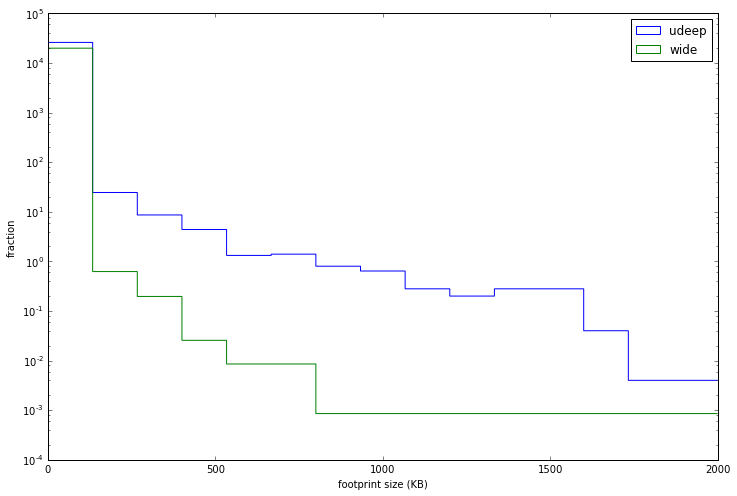
\includegraphics[width=\textwidth]{histogram.png}
\caption{Histogram of per-\Object storage costs for \texttt{HeavyFootprints} in LSST processing of HSC SSP data.}
\label{fig:histogram}
\end{figure}

It is also worth noting that the dynamic range of per-\Object \texttt{HeavyFootprint} storage sizes spans several orders of magnitude, as shown in Figure~\ref{fig:histogram}.  Storage cannot be assumed to be even approximately constant across \Objects.

\bibliographystyle{gaia_aa}
\bibliography{lsst,local-refs}

\end{document}
